% Source: AESP_466_ClassWork/Supplements/Notes/latex/2.2/2.2.tex

\documentclass[border=4pt]{standalone}
\usepackage{amsmath,amssymb,amsthm}
\usepackage{graphicx}
\usepackage{tikz}
\usepackage{xcolor}
\usetikzlibrary{arrows.meta,calc,positioning,decorations.markings,patterns,shapes.geometric,angles,quotes,3d}

\definecolor{Garnet}{HTML}{73000A}
\definecolor{USC_Rose}{HTML}{CC2E40}
\definecolor{USC_Blue}{HTML}{466A9F}
\definecolor{USC_Slate}{HTML}{1F414D}
\definecolor{USC_Olive}{HTML}{65780B}
\definecolor{USC_Lime}{HTML}{CED318}
\definecolor{USC_Gold}{HTML}{A49137}
\definecolor{USC_Black90}{HTML}{565556}
\definecolor{USC_Black10}{HTML}{ECECEC}

\newcommand{\vect}[1]{\mathbf{#1}}
\newcommand{\mat}[1]{\mathbf{#1}}
\newcommand{\uvec}[1]{\hat{\mathbf{#1}}}
\newcommand{\transpose}{^{\mkern-1.5mu\mathsf{T}}}
\newcommand{\inv}{^{-1}}
\newcommand{\deriv}[2]{\frac{d #1}{d #2}}
\newcommand{\pderiv}[2]{\frac{\partial #1}{\partial #2}}

\begin{document}
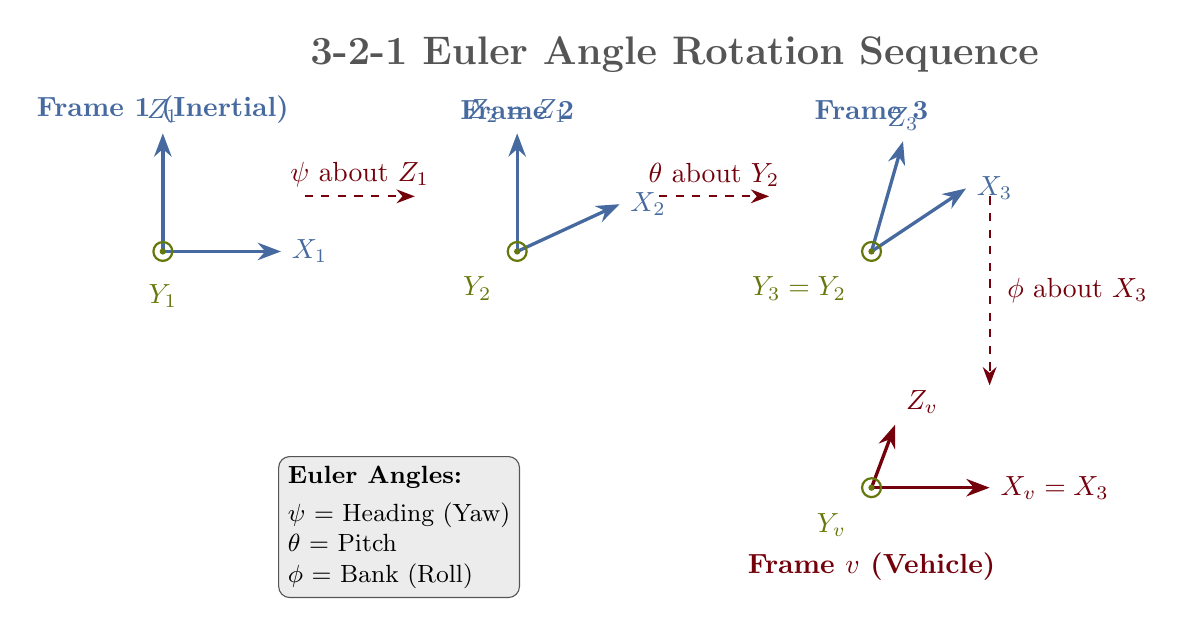
\begin{tikzpicture}[>=Stealth, scale=1.0]
    % Title
    \node[font=\Large\bfseries, USC_Black90] at (6.5,5.5) {3-2-1 Euler Angle Rotation Sequence};

    % Frame 1 (Inertial)
    \begin{scope}[shift={(0,3)}]
        \node[font=\bfseries, USC_Blue] at (0,1.8) {Frame 1 (Inertial)};
        \draw[->, very thick, USC_Blue] (0,0) -- (1.5,0) node[right] {$X_1$};
        \draw[->, very thick, USC_Blue] (0,0) -- (0,1.5) node[above] {$Z_1$};
        \draw[thick, USC_Olive] (0,0) circle (0.12);
        \fill[USC_Olive] (0,0) circle (0.04);
        \node[USC_Olive, below] at (0,-0.3) {$Y_1$};

        % Rotation arrow
        \draw[->, thick, Garnet, dashed] (1.8,0.7) -- (3.2,0.7);
        \node[Garnet, above] at (2.5,0.7) {$\psi$ about $Z_1$};
    \end{scope}

    % Frame 2 (after yaw)
    \begin{scope}[shift={(4.5,3)}]
        \node[font=\bfseries, USC_Blue] at (0,1.8) {Frame 2};
        \draw[->, very thick, USC_Blue] (0,0) -- (1.3,0.6) node[right] {$X_2$};
        \draw[->, very thick, USC_Blue] (0,0) -- (0,1.5) node[above] {$Z_2 = Z_1$};
        \draw[thick, USC_Olive] (0,0) circle (0.12);
        \fill[USC_Olive] (0,0) circle (0.04);
        \node[USC_Olive, below left] at (-0.2,-0.2) {$Y_2$};

        % Rotation arrow
        \draw[->, thick, Garnet, dashed] (1.8,0.7) -- (3.2,0.7);
        \node[Garnet, above] at (2.5,0.7) {$\theta$ about $Y_2$};
    \end{scope}

    % Frame 3 (after pitch)
    \begin{scope}[shift={(9,3)}]
        \node[font=\bfseries, USC_Blue] at (0,1.8) {Frame 3};
        \draw[->, very thick, USC_Blue] (0,0) -- (1.2,0.8) node[right] {$X_3$};
        \draw[->, very thick, USC_Blue] (0,0) -- (0.4,1.4) node[above] {$Z_3$};
        \draw[thick, USC_Olive] (0,0) circle (0.12);
        \fill[USC_Olive] (0,0) circle (0.04);
        \node[USC_Olive, below left] at (-0.2,-0.2) {$Y_3 = Y_2$};
    \end{scope}

    % Arrow from Frame 3 to Frame V
    \draw[->, thick, Garnet, dashed] (10.5,3.7) -- (10.5,1.3);
    \node[Garnet, right] at (10.6,2.5) {$\phi$ about $X_3$};

    % Frame V (Vehicle/Body frame)
    \begin{scope}[shift={(9,0)}]
        \node[font=\bfseries, Garnet] at (0,-1.0) {Frame $v$ (Vehicle)};
        \draw[->, very thick, Garnet] (0,0) -- (1.5,0) node[right] {$X_v = X_3$};
        \draw[->, very thick, Garnet] (0,0) -- (0.3,0.8) node[above right] {$Z_v$};
        \draw[thick, USC_Olive] (0,0) circle (0.12);
        \fill[USC_Olive] (0,0) circle (0.04);
        \node[USC_Olive, below left] at (-0.2,-0.2) {$Y_v$};
    \end{scope}

    % Summary box
    \node[draw=USC_Black90, fill=USC_Black10, rounded corners, align=left, font=\small] at (3,-0.5) {
        \textbf{Euler Angles:}\\[0.3em]
        $\psi$ = Heading (Yaw)\\
        $\theta$ = Pitch\\
        $\phi$ = Bank (Roll)
    };
\end{tikzpicture}
\end{document}
